\section{Durchführung}
\label{sec:Durchführung}
Der Versuch besteht aus einer Kupfer-Röntgenröhre mmit einem LiF-Kristall und einem Geiger-Müller-Zählrohr. Im folgenden Versuch werden alle Spektren aufgezeichnet.
Vor das Geiger-Müller-Zählrohr werden Blenden mit Absorbern unterschiedlicher Elemente gesteckt. Der Versuchsaufbau ist in \autoref{fig:aufbau} abgebildet.
\begin{figure}[H]
    \centering
    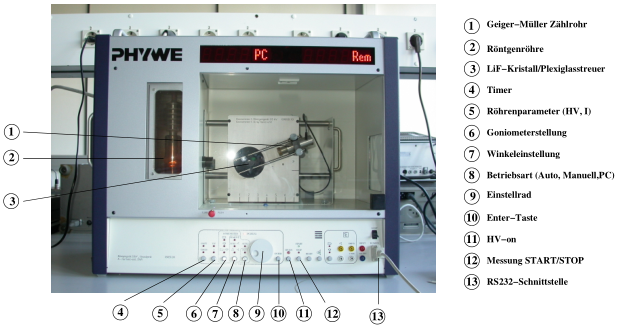
\includegraphics[width = 0.4 \textwidth]{data/aufbau.png}
    \caption{Versuchsaufbau zur Messung von Röntgenemission und -absorption \cite{Anleitung602}.}
    \label{fig:aufbau}
\end{figure}